\section{Rewrite Rules}%
\label{rewrite-rules}

\subsection{Spider Fusion}%
The most fundamental rule of the ZX calculus is the \textit{spider fusion} rule \cite{Wetering2020}. It states that two spiders connected by one or more wires fuse if they are the same colour. It is the generalisation of adding the phases of successive rotations of the Bloch sphere. Since we interpret the phases $\alpha$ and $\beta$ as $e^{i\alpha}$ and $e^{i\beta}$, it follows that the phase $\alpha + \beta$ is modulo $2\pi$.

\begin{figure}[H]
    \centering
    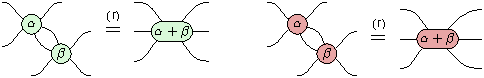
\includegraphics[width=0.75\textwidth]{chapter-2/fusion}
    \caption{Spider fusion rule for $Z$ spiders (left) and $X$ spiders (right).}
    \label{spider-fusion}
\end{figure}

We can use this rule to identify commutation relations such as $Z$ rotations commuting through CNOT controls, and $X$ rotations, through CNOT targets.

% \vspace{5pt}
\includezxdiagram{chapter-2/cnot_commutation}{0.8}

%%%

\subsection{Identity Removal}%

The \textit{identity removal} rule states that any two-legged spider with no phase ($\alpha = 0$) is equivalent to a rotation by 0 radians, or identity.

\begin{figure}[H]
    \centering
    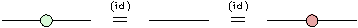
\includegraphics[width=0.6\textwidth]{chapter-2/identity}
    \caption{Identity removal rule.}
    \label{identity}
\end{figure}

Combining this with the spider fusion rule (\ref{spider-fusion}), we see that two successive rotations with opposite phases is equivalent to an empty wire.

\includezxdiagram{chapter-2/cancelling_rotations}{0.7}

%%%

\subsection{State Copy and $\pi$ Copy Rules}%

We can depict the $Z$ and $X$ eigenstates by assigning a phase to a $Z$ or an $X$ spider, respectively, through a Boolean variable $a$ (0 or 1) multiplied by $\pi$ \cite{Wetering2020}.

\includezxdiagramtext{chapter-2/boolean_x}{0.075}{
\ket 0 \text{ where $a = 0$ and }
\ket 1 \text{ where $a = 1$}}
%
\includezxdiagramtext{chapter-2/boolean_z}{0.075}{
\ket + \text{ where $a = 0$ and }
\ket - \text{ where $a = 1$}}

The $\pi$ \textit{copy} rule states that when a Pauli $Z$ or Pauli $X$ gate is pushed through a spider of the opposite colour, it is copied on all other legs and negates the spider's phase. A similar \textit{state copy} rule applies to the $Z$ and $X$ eigenstates.

\begin{figure}[H]
    \centering
    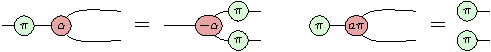
\includegraphics[width=0.8\textwidth]{chapter-2/pi_state_copy}
    \caption{$\pi$ copy (left) and state copy (right) rules for Pauli $Z$ gate and $Z$ eigenstates.}
    \label{state-copy}
    \label{pi-copy}
\end{figure}

%%%

\subsection{Hadamard Copy Rule}%
\label{hadamard-copy}

Similarly, the Hadamard copy rule states that when a Hadamard gate is pushed through a Pauli 

%%%

\subsection{Bialgebra Rule}%
Using the spider fusion rule (\ref{spider-fusion}), we can show that a spider with two inputs and one output behaves like a classical XOR gate when applied to the eigenstates of the \textit{same} basis. Whilst using the state copy rule (\ref{state-copy}), we can show that a spider with one input and two outputs behaves like a classical COPY gate when applied to the eigenstates of the \textit{opposite} basis.

\begin{figure}[H]
    \centering
    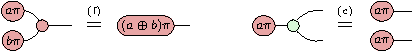
\includegraphics[width=0.7\textwidth]{chapter-2/xor_copy}
    \caption{XOR gate (left) and COPY gate (right) with respect to the $Z$ eigenstates.}
    \label{xor}
    \label{copy}
\end{figure}

Hence, using the natural commutation relation of the classical XOR and COPY gates, we define the \textit{bialgebra} rule. We encourage the reader to verify this relation.

\begin{figure}[H]
    \centering
    \includezxdiagram{chapter-2/bialgebra}{1}
    \caption{The bialgebra rule (and its classical motivation).}
    \label{bialgebra}
\end{figure}

%%%

\subsection{Hopf Rule}%

Like with the bialgebra rule, our motivation for this rule is classical. Copying two bits then taking their XOR invariably yields 0. Hence, we define the Hopf rule.

\includezxdiagram{chapter-2/hopf}{1}%
\label{hopf}

